\chapter{Ley de Gravitación Universal}

\begin{miparrafo}
\begin{multicols}{2}
En la antigüedad, se observó que la órbita de Marte describía la trayectoria que aparece en la figura. Las órbitas no eran pues circulares tal como imaginaban. Fue Ptolomeo (s. II) quien describió este movimiento, suma de rotación y traslación, como \emph{epicicloide}.
\begin{figure}[H]
	\centering
	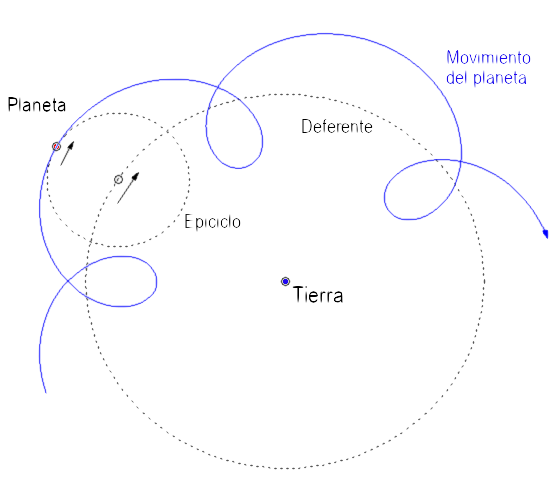
\includegraphics[width=.5\textwidth]{imagenes/imagenes14/T14IM01.png}
\end{figure}
\end{multicols}
\vspace{-10mm} %****************************************
A medida que avanzaron las técnicas de astronómicas observación (telescopio de Galileo) se vieron confirmadas las teorías de Ptolomeo.

Allá por el XV, Copérnico (final de la edad media, principio del renacimiento) niega que el centro del Universo sea la Tierra, por lo que le tacharían de hereje; sus teorías eran peligrosas para el orden establecido.

Cuando Newton enfocó su telescopio a Júpiter y vio cuatro satélites girando a su alrededor se afianzan las teorías de Copérnico y empiezan a perder importancia las creencias.

Copérnico planteó un sistema solar como hoy lo conocemos, con el Sol en su centro (visión heliocentrista, concebida en primera instancia por Aristarco de Samos --s. III a.C.-- frente a la geocentrista). Sus teorías fueron comprobadas por los estudios de momentos angulares de planetas que realizó Kepler (s. XVII) y matemáticamente por Tycho Brahe. Más tarde, Newton, introduciría los conceptos de aceleración, fuerza y campo central.

Las tres leyes de Kepler

Kepler accedió a los datos de las órbitas de los planetas que durante años se habían ido recolectando por Tycho Brahe que se centró en Marte, con una órbita elíptica muy acusada. De otra manera le hubiera sido imposible a Kepler darse cuenta de que las órbitas de los planetas eran elípticas. Inicialmente, Kepler intentó la circunferencia por ser la más perfecta de las trayectorias, pero los datos observados impedían un ajuste correcto, lo que entristeció a Kepler, ya que no podía saltarse un pertinaz error de ocho minutos de arco. Kepler comprendió que debía abandonar la circunferencia, lo que implicaba abandonar la idea de un "mundo perfecto". De profundas creencias religiosas, le costó llegar a la conclusión de que la tierra era un planeta imperfecto, asolado por las guerras. En esa misma misiva incluyó la cita clave: "Si los planetas son lugares imperfectos, ¿por qué no han de serlo las órbitas de los mismos?". Finalmente utilizó la fórmula de la elipse, una rara figura descrita por Apolonio de Pérgamo (s. III a.C.)  y descubrió que encajaba perfectamente en las mediciones de Tycho.

Había descubierto su primera ley, la primera ley de Kepler:

\emph{1.- Los cuerpos celestes tienen movimientos elípticos alrededor del Sol, estando éste situado en uno de los dos focos que tiene la elipse.}

Pasó a comprobar la velocidad del planeta a través de las órbitas llegando a la segunda ley:
\begin{multicols}{2}
\begin{figure}[H]
	\centering
	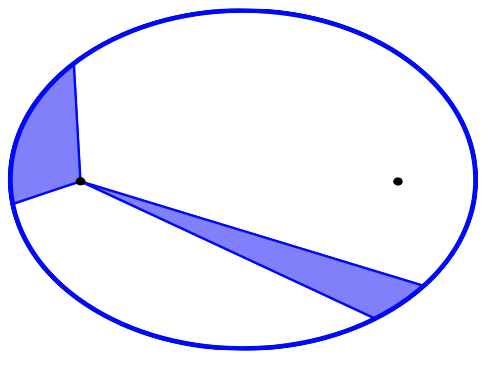
\includegraphics[width=.35\textwidth]{imagenes/imagenes14/T14IM02.png}
\end{figure}
\emph{2.-  El radio vector que une un planeta y el Sol recorre áreas iguales en tiempos iguales.}

Durante mucho tiempo, Kepler sólo pudo confirmar estas dos leyes en el resto de planetas. Aun así fue un logro espectacular, pero faltaba relacionar las trayectorias de los planetas entre sí. Tras varios años, descubrió la tercera ley e importantísima ley del movimiento planetario:
\end{multicols}
\emph{3.-  Para cualquier planeta, el cuadrado de su período orbital es directamente proporcional al cubo de la longitud del semieje mayor de su órbita elíptica. $T/a^3=cte$}

Esta ley, llamada también ley armónica, junto con las otras leyes, permitía ya unificar, predecir y comprender todos los movimientos de los astros.
\end{miparrafo}

\section{Ley de Gravitación Universal}

Disponemos de $N$ cuerpos que se mueven produciendo variaciones y fluctuaciones, pero nos limitaremos a estudiar el problema de dos cuerpos sometidos a la fuerza de un campo exterior.

Sabemos que, del tema anterior: $\ \displaystyle \mu \dv[2]{\vec r_{12}}{t} \ = \ \vec F_{12} \ + \ \mu \left[ \dfrac {\vec F_1^{(e)}}{m_1}-\dfrac {\vec F_2^{(e)}}{m_2} \right]$

Exigíamos que $\dfrac {\vec F_i^{(e)}}{m_i}=\overrightarrow{cte}$, con lo que el corchete anterior se anula y se obtiene, precindiendo de los subíndices:


$$  \displaystyle \mu \dv[2]{\vec r}{t} \ = \ \vec F\ ; \quad r^2 \dv{\theta}{t}=\dfrac L \mu=cte  \ \to \ \  \dv{S}{t}=\dfrac 1 2 \dfrac L \mu = cte$$


Vamos a pasar la ecuación $\mu \dv[2]{\vec r}{t}=\vec F$ a coordenadas polares:

$\displaystyle \left[ \dv[2]r{}{t}- r\left(\dv{\theta}{t} \right)^2\right]\vec u_r + \left[ 2 \dv{r}{t}\dv{\theta}{t}+r\dv[2]{\theta}{t} \right]\vec u_\theta = \dfrac F \mu \vec u_r$

\vspace{3mm} %*************************************
\begin{multicols}{2}
$\quad$

La fuerza es el la dirección $\vec u_r$, no hay fuerza en la dirección $\vec u_\theta$.
\begin{figure}[H]
	\centering
	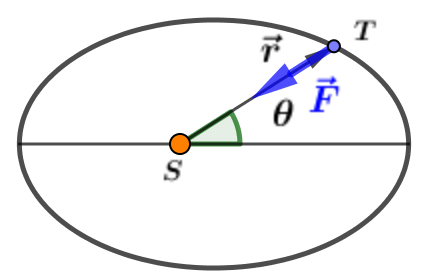
\includegraphics[width=.3\textwidth]{imagenes/imagenes14/T14IM04.png}
\end{figure}
\end{multicols}

Podemos extraer dos ecuaciones escalares:

$$\displaystyle \dv[2]{r}{t}- r\left(\dv{\theta}{t} \right)^2 =\dfrac F \mu \ ; \qquad  \qquad  2 \dv{r}{t}\dv{\theta}{t}+r\dv[2]{\theta}{t}=0 $$

De la segunda ecuación, multiplicando ambos términos por $r$:

$\displaystyle 2r \dv{r}{t}\dv{\theta}{t}+r^2\dv[2]{\theta}{t}= \dv{t}\left[r^2 \dv{\theta}{t} \right] =0  \quad \to \quad \boldsymbol{r^2\  \dv{\theta}{t}\ =\ cte}$

Trabajemos ahora con el otro término: $\displaystyle \dv[2]{r}{t}- r\left(\dv{\theta}{t} \right)^2 =\dfrac F \mu $

\vspace{3mm} %**********************************************
\textcolor{gris}{\rule{60mm}{0.4pt}
\hspace{5mm} Inciso matemático: la elipse.}
\begin{multicols}{2}
$r+r'=2a \to r'=2a-r$

Th. coseno: $r'^2=r^2+4c^2-4rc\cos \theta$

Luego: $(2a-r)^2=r^2+4c^2-4rc\cos \theta$	

$4a^2 + \cancel{r^2} -4ar=\cancel{r^2}+4c^2-4rc\cos \theta$

$4a^2  -4ar=4c^2-4rc\cos \theta$

De donde: $\ a^2-c^2=r(a-\cos \theta)$
\begin{figure}[H]
	\centering
	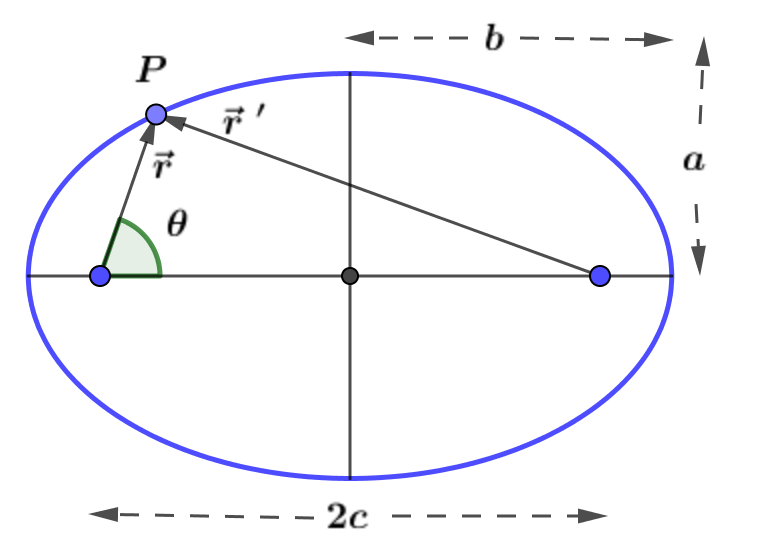
\includegraphics[width=.45\textwidth]{imagenes/imagenes14/T14IM05.png}
\end{figure}
\end{multicols}

Como $a^2-c^2=b^2 \to b^2=ra\left(1-\dfrac c a \cos \theta \right)$

Se llama \emph{excentricidad} o achatamiento de la elipse a la cantidad $\boldsymbol{ \epsilon=\dfrac c a }$

$\boldsymbol{ \ l \ = \dfrac{b^2}{a}=r\left(1-\epsilon \cos \theta \right) }$

\textcolor{gris}{ Fin inciso matemático. \hspace{5mm} \rule{67mm}{0.4pt} }
\vspace{3mm} %**********************************************

Seguimos con nuestro problema.

$l =\dfrac{b^2}{a}=r\left(1-\epsilon\cos \theta \right) \to \epsilon \cos \theta=1-\dfrac l r $, 

derivando respecto de $t$, varían $r$ y $\theta$,

$\displaystyle -\epsilon \sin \theta \dv{\theta}{t}  = - \dfrac{l}{ r^2 } \dv{r}{t}\ \to \ \displaystyle -\epsilon \sin \theta = - \dfrac{l}{ r^2 \dv{\theta}{t} } \dv{r}{t}\ \ $, como $\displaystyle r^2 \dv{\theta}{t}=\dfrac {L_{CM}}{\mu}$

$\displaystyle \epsilon \sin \theta =\dfrac{l\ \mu}{L_{CM}}\ \dv{r}{t} \ \to \ \ \dv{r}{t}=\dfrac {\epsilon \ L_{CM} \sin \theta}{\mu \ l}$

Volviendo a derivar:
$\ \ \displaystyle \dv[2]{r}{t}=-\dfrac {\epsilon L_{CM}}{\mu \ l}\cos \theta \dv{\theta}{t} $

Sustituyendo $\displaystyle \ \epsilon \cos \theta = 1-\dfrac l r\ $ y $\ \displaystyle \dv{\theta}{t}=\dfrac {L_{CM}}{\mu\ r^2}$ en la exprersión anterior:

$\displaystyle \dv[2]{r}{t}=\dfrac { L_{CM}}{\mu \ l} \left( \dfrac l r - 1 \right) \dfrac {L_{CM}}{\mu\ r^2} \ = \ \dfrac{L^2_{CM}}{\mu^2\ r^3} - \dfrac{L^2_{CM}}{\mu^2\ r^2\ l}$

Sustituyendo lo encontrado en $\ \displaystyle \dv[2]{r}{t}-r \left( \dv{\theta}{t} \right)^2=\dfrac L \mu \ $ y teniendo en cuenta que $\displaystyle \dv{\theta}{t}=\dfrac {L_{CM}}{\mu\ r^2}$, obtenemos:

$\displaystyle \ \cancel{\dfrac{L^2_{CM}}{\mu^2\ r^3}} - \dfrac{L^2_{CM}}{\mu^2\ r^2\ l}-\cancel{r\dfrac {L^2_{CM}}{\mu^2\ r^4}}=\dfrac F \mu$


$$\displaystyle - \dfrac{L^2_{CM}}{\cancel{\mu} \ r^2 \ l}=\dfrac F {\cancel{\mu}} \quad \to \qquad \boldsymbol{F\ = \ - \dfrac {c}{r^2}} \qquad \text{con\ } c=\frac{L^2_{CM}}{\mu\ l}=cte$$
 
Vectorialmente: 

\begin{equation}
\boldsymbol{
\overrightarrow{F} \ = \ -\dfrac c{r^2} \ \vec u_r
}
\end{equation}
\begin{miparrafodestacado}
La fuerza que ejercen entre sí dos cuerpos en atractiva ($-$) e inversamente proporcional al cuadrado de la distancia.	
\end{miparrafodestacado}

Para determinar el modo en que $F$ depende de $r^2$, Newton estableció un 
\emph{postulado}: ``la fuerza también varia con la masa de los cuerpos y, para todas las sustancias, se cumple que:

\begin{equation}
\subrayado {\  \boxed { \boldsymbol { 
\ \overrightarrow  F \ = \ - G\ \dfrac {M\ m}{r^2} \ \vec u_r \ 
} } \ }	
\end{equation}
\centerline{\emph{\textbf{Ley de Gravitación Universal de Newton}}}

\vspace{10mm} %**********************************************************
\section[Verificación de la tercera ley de Kepler]{Verificación de la tercera ley de Kepler\sectionmark{Tercera ley de Kepler}}
\sectionmark{Tercera ley de Kepler}

\emph{El cuadrado de los periodos de revolución es igual al cubo de los semiejes mayores.}


Tenemos que $\quad \dfrac {L^2_{CM}}{\mu\ l}\ = \ c\ = \ G\ M\ m$

$l=\dfrac b a\ , \quad \text{ con } b=\text{semieje mayor y }c=\text{semieje menor}$

$L^2_{CM}=c\mu l=GMm\mu l=G\mu M m \dfrac {b^2}{a}; \quad \mu=\dfrac{mM}{m+M} \quad \to $

$\to \quad  L^2_{CM}=G\mu^2 (M+m) \dfrac {b^2}{a}$, expresión que usaremos más adelante.

Ley áreas Kepler: $\displaystyle \quad \dv{S}{t}=\dfrac 1 2 \dfrac {L_{CM}}{\mu} \to \int_0^S \dd S = \int_0^T \dfrac 1 2 \dfrac {L_{CM}}{\mu} \ \dd t \ \to $

$\displaystyle \to \quad S= \dfrac 1 2 \dfrac{L_{CM}}{\mu}\cdot T$

\vspace{35mm} %**********************************************
\textcolor{gris}{\rule{50mm}{0.4pt} \hspace{5mm} Inciso matemático: área de la elipse.}
\begin{multicols}{2}
\begin{figure}[H]
	\centering
	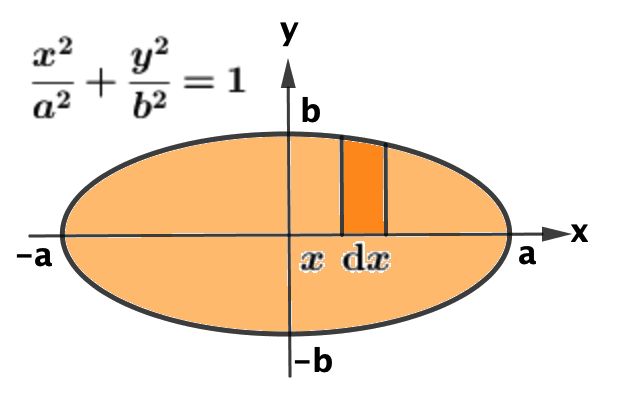
\includegraphics[width=.5\textwidth]{imagenes/imagenes14/T14IM06.png}
\end{figure}
$\dfrac {x^2}{a^2}+\dfrac{y^2}{b^2}=1 \ \to \ y=b\ \sqrt{1-\dfrac{x^2}{a^2}};\quad S=2 \int y \dd x = \displaystyle 2\int_{-a}^{a} b\  \sqrt{1-\dfrac{x^2}{a^2}} \ \dd x$
\end{multicols}

Cambio de variable: $\dfrac x a =\sin t \to \begin{cases}
\ \dd x= a \cos t \dd t \\
x=a \ \ \to \sin t = 1\ \  \to t=\pi/2 \\
x=-a \to \sin t = -1 \to t=-\pi/2  	
 \end{cases}$

$\displaystyle S = 2 \int_{-\pi/2}^{\pi/2} b \sqrt{1-\sin^2 t}\ a \cos t\ \dd t=2ab\int_{-\pi/2}^{\pi/2} \cos^2 t\ \dd t$

Trigonometría, ángulo doble: $	\cos^2 t =\dfrac{1+\cos 2t}{2}$, luego

$\displaystyle S=\cancel{2} \int_{-\pi/2}^{\pi/2} \dfrac{1+\cos 2t}{\cancel{2}}\ \dd t = ab {\left[ t+\dfrac {\sin 2t}{2} \right]}_{-\pi/2}^{\pi/2} =\pi \ a \ b$

\textcolor{gris}{ Fin inciso matemático. \hspace{5mm} \rule{67mm}{0.4pt} }
\vspace{3mm} %**********************************************

Siguiendo con lo que teníamos, $\ \displaystyle  S= \dfrac 1 2 \dfrac{L_{CM}}{\mu}\cdot T \  \to \ \ \pi \ a \ b = \dfrac 1 2 \dfrac{L_{CM}}{\mu}\cdot T$

$T^2 = \dfrac{4 \pi^2 a^2 b^2 \mu^2}{L^2_{CM}} $ junto con la expresión anterior $\ L^2_{CM}=G\mu^2 (M+m) \dfrac {b^2}{a}$

\begin{equation}
\boldsymbol{ T^2 } = \dfrac{4 \pi^2 a^2 b^2 \mu^2 a}{G \mu^2 (M+m) b^2} =  \boldsymbol{ \dfrac {4\pi^2}{G(M+m)} \cdot a^3 }
\end{equation}

cqd: los cuadrados de los periodos de revolución son proporcionales a los cubos de los semiejes mayores (Newton realizó este razonamiento al revés que nosotros).

`!Un momento!: nosotros exigimos que la constante de proporcionalidad fuese la misma para todos los planetas y $M+m$ no lo es, depende de la masa del planeta $m$.

?`Cuál es la contradicción?: resulta que $M>>m$, por lo que $m$ es despreciable frente a $M$ y, entonces, sí que es \emph{aproximadamente} constante, se comete un error pequeño.

\section[Energía potencial gravitatoria. Campo gravitatorio. Potencial gravitatorio]{Energía potencial gravitatoria. Campo gravitatorio. Potencial gravitatorio\sectionmark{Potencial gravitatorio}}
\sectionmark{Potencial gravitatorio}

Como $\ \overrightarrow  F \ = \ - G\ \dfrac {M\ m}{r^2} \ \vec u_r \ $, la fuerza en \emph{central}, luego es conservativa y, por ello, deriva de un potencial escalar.

$\displaystyle \vec F=-\overrightarrow{\grad} \mathcal E_p;\qquad \overrightarrow{\grad}=\vec u_r \ \dv{r};\qquad \vec F=-\vec u_r \dv{\mathcal E_p}{r}=-\vec u_r \ G\ \dfrac {M\ m}{r^2} $

$\displaystyle \dv{\mathcal E_p}{r}= \ G\ \dfrac {M\ m}{r^2} \quad \to \qquad \int_{\mathcal E_p(r_1)}^{\mathcal E_p(r_2)} \dd \mathcal E_p=\int_{r_1}^{r_2} G \dfrac {Mm}r^2 \dd r  $ 

Luego $\ \ \mathcal E_p(r_2) - \mathcal E_p(r_1)=-GMm\left(\dfrac 1 {r_2^2}-\dfrac 1{r_1^2} \right)$

Establecemos la constante de la energía potencial exigiendo que $\mathcal E_p(\infty)=0$ \textcolor{gris}{$\displaystyle \ \lim_{r\to \infty}\mathcal E_p(r)=0$}. Con ello, tenemos que

\begin{equation}
	\subrayado{\ \boldsymbol{\mathcal E_p(r)=-\dfrac{G\ M\ m}{r}}\ }
\end{equation}

$r$ es la distancia al punto en que se calcula la energía potencial desde el centro de masas, $CM$

$\vec F$ lo podemos asociar a la acción de un \emph{campo} $\vec E$, de modo que $\vec F=m\vec E$. Podremos escribir que:

\begin{equation}
	\subrayado{\ \boldsymbol{\vec E=-\dfrac {G\ M}{r^2} \ \vec u_r}\ }
\end{equation}

El potencial gravitatorio $V$ que crea una masa puntual $M$ es $\ \vec E=-\overrightarrow{\grad} V \ \to \ V=-\dfrac {GM}{r}\ $, un escalar.

\begin{multicols}{2}
El concepto de potencial gravitatorio es muy útil cuando se considera más de una fuente puntual gravitatoria: 

$\displaystyle V=-G \sum_i \dfrac {M_i}{r_i}$
\begin{figure}[H]
	\centering
	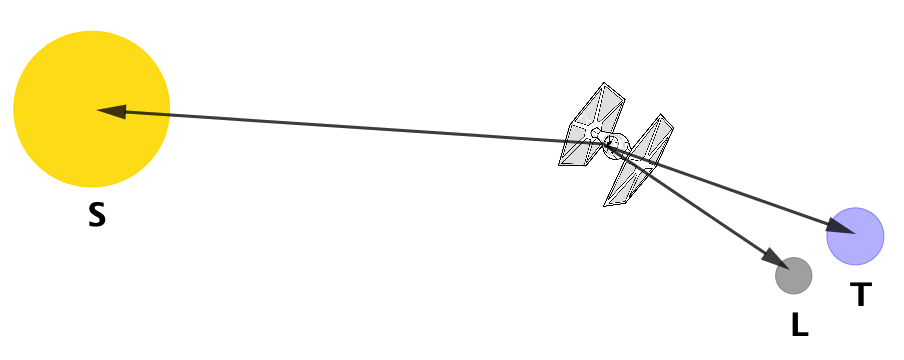
\includegraphics[width=.55\textwidth]{imagenes/imagenes14/T14IM08.png}
\end{figure}
\end{multicols}

\begin{figure}[H]
	\centering
	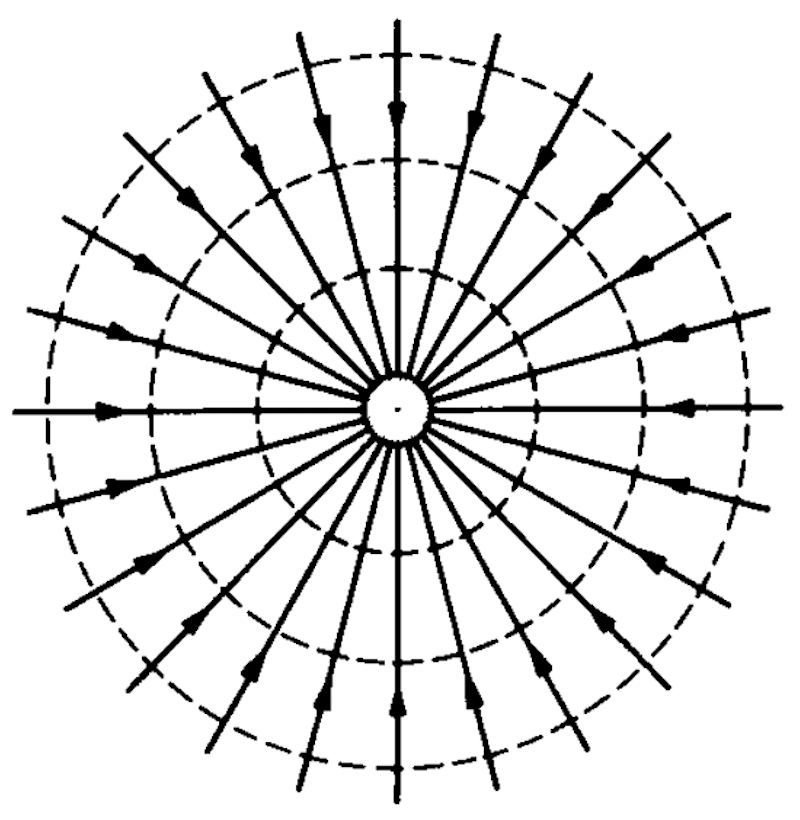
\includegraphics[width=.5\textwidth]{imagenes/imagenes14/T14IM09.png}
	\caption*{Línea de fuerza y superficies equipotenciales del campo gravitatorio producido por una masa puntual.}
\end{figure}

\section{Campo gravitatorio debido a un cuerpo esférico}

Eliminamos la simplificación que hacíamos has ahora de considerar las masas puntuales. Supongamos que tenemos un cuerpo esférico hueco, con toda su masa distribuida uniformemente sobre su superficie y estudiaremos el campo gravitatorio que produce.

\begin{figure}[H]
	\centering
	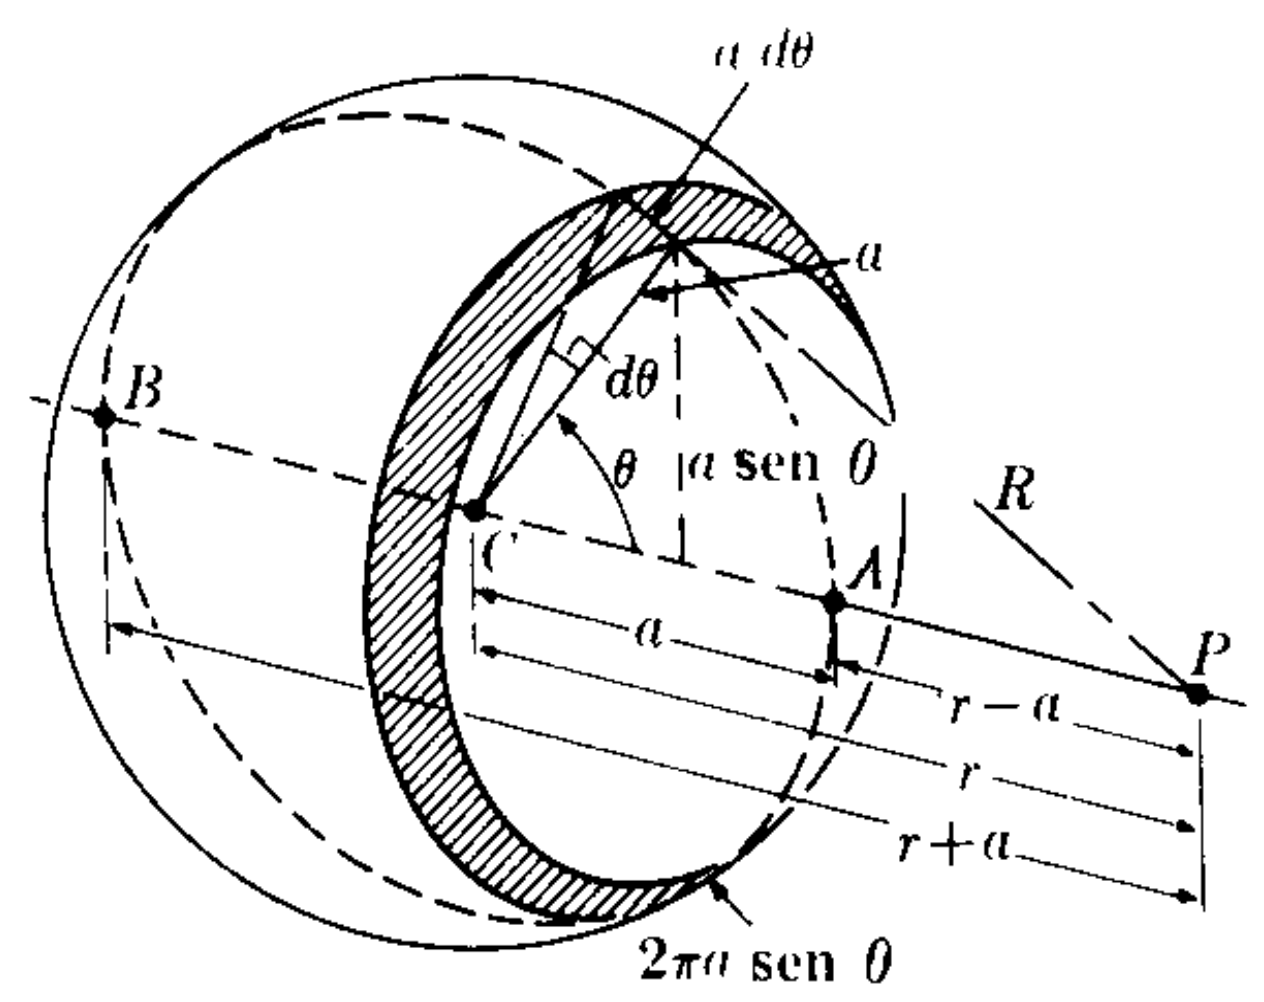
\includegraphics[width=.75\textwidth]{imagenes/imagenes14/T14IM10.png}
\end{figure}

Elemento de área de la esfera.

$\dd S= (a\dd \theta)\cdot (2\pi a \sin \theta)=2\pi a^2 \sin \theta \ \dd \theta$

Masa del elemento de área: la masa está distribuida uniformemente en la superficie esférica:

$\dd m=\dfrac m{4\pi a^2}\cdot 2\pi a^2 \sin \theta \dd \theta = \dfrac{m \sin \theta \ \dd \theta}2$

Como $\displaystyle V=-G \sum_i \dfrac {m_i}{r_i}$, el potencial gravitatorio que esta masa elemental $\dd m$ crea en un punto $P$ será:

$\dd V =- G \dfrac{m \sin \theta \ \dd \theta}{2R} \quad \Rightarrow$

Geometría del dibujo, teorema del coseno: $R^2=r^2+a^2-2aR\cos \theta$

$a, R = ctes \ \to \ 2R \ \dd R=2ar \ \dd r \cos \theta \ \to \ \sin \theta \ \dd \theta =\dfrac {R \ \dd R}{ar}$, por lo que:

$\Rightarrow \quad \dd V=-G\dfrac{m R \dd R}{2aRr}=-\dfrac{Gm}{2ar} \ \dd R \ \to $

$\to \  V=-\dfrac{Gm}{2ar} \displaystyle \int_{r-a}^{r+a} \ \dd R 
=-\dfrac{Gm}{2ar} \ \eval{ R }_{r-a}^{r+a}= -\dfrac{Gm}{r} $

El potencial creado por una esfera hueca de masa $m$ a una distancia al centro $r$ de un punto situado es su exterior es:

$$\boldsymbol{ V \ = \  -\dfrac{Gm}{r}};  \qquad \boldsymbol{ \vec E=-}\overrightarrow{\grad} V =-\vec u_r \ \displaystyle \dv{V}{r} \boldsymbol{ = -\dfrac{Gm}{r^2} \ \vec u_r}; \qquad r\geq a$$

Si $P$ está dentro de la esfera, $r<a$, los límites de integración serán $a+r$ y $a-r$, por lo que:
$V=-\dfrac{GM}{2ar} \displaystyle \int_{a-r}^{a+r} \dd R
=-\dfrac{GM}{a}=cte;\quad r<a$

Tenemos un potencial gravitacional independiente de $P$. Al ser cte. $\ \vec E =\vec 0,\ r<a$

Resumiendo:

$$\boldsymbol{
V=\begin{cases}
-\dfrac{GM}{a}=cte & r<a \\ \\ 
-\dfrac{GM}{r} & r\geq a	
\end{cases} \ \rightarrow \ 
\ \vec E=
\begin{cases}
	\qquad \vec 0 & r<a \\ \\ 
	-\dfrac{GM}{r^2}\ \vec u_r & r\geq a	
\end{cases}
}$$


------ ?`A qué conclusión se puede llegar?

\emph{El campo gravitatorio y el potencial, en un punto exterior a una masa uniformemente distribuida en una capa esférica es \textbf{como si} se tratase del campo y potencial gravitatorios de una partícula de la misma masa situada en el centro de la esfera. En puntos del interior de la capa esférica, el campo es cero y el potencial constante.}

\begin{figure}[H]
	\centering
	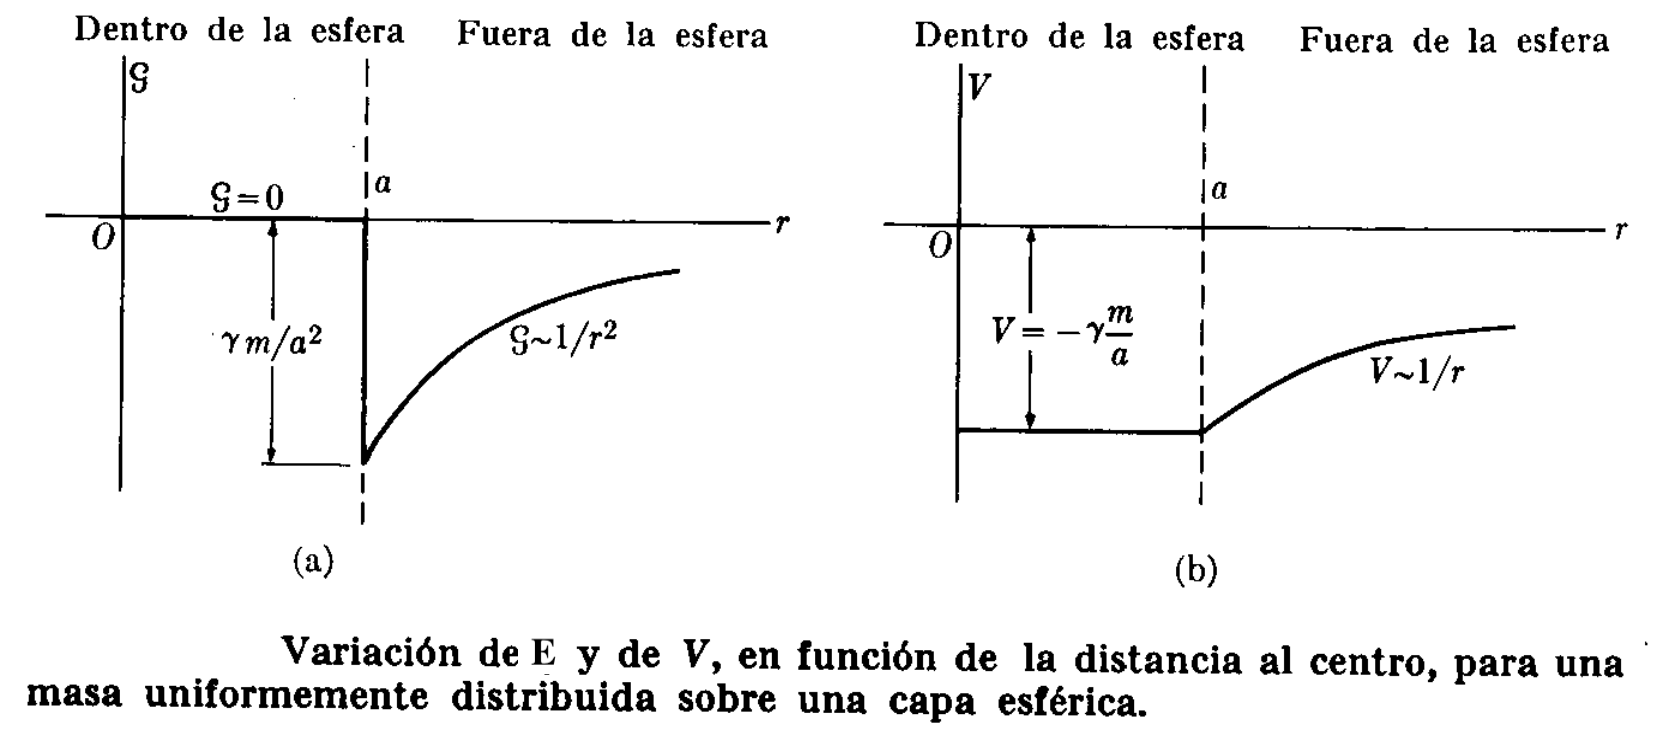
\includegraphics[width=.75\textwidth]{imagenes/imagenes14/T14IM13.png}
\end{figure}

------ Pero, ?`qué ocurre con una esfera maciza (toda la masa distribuida homogéneamente en su volumen)?

En este caso, podemos considerar la esfera maciza como una serie de capas de esferas huecas de masa $m_i$ igual en todas las capas.

$\displaystyle V=-G \sum_i \dfrac {m_i}{r_i} =-\dfrac G r \sum_i m_i = -\dfrac G r M_T \ \to \vec E=-\dfrac {GM_T} r \ \vec u_r $

\begin{multicols}{2}
También \emph{el potencial y el campo gravitatorio creado por una esfera maciza en un punto exterior a ella es como el creado por una masa puntual}.
\begin{figure}[H]
	\centering
	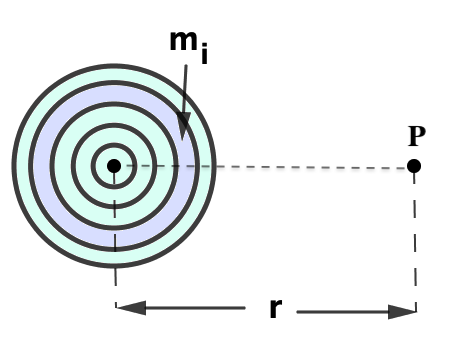
\includegraphics[width=.3\textwidth]{imagenes/imagenes14/T14IM11.png}
\end{figure}	
\end{multicols}

Para el campo en el interior de una esfera homogénea, es decir, cuando $P$ está a distancia $r<a$, las capas con $r>a$ no contribuyen al campo. El campo resultante de todas las capas con $r\leq a$ produce un efecto \emph{como si} se tratase de una masa puntual $m'$ correspondiente a estas capas internas y situada en el centro de la circunferencia.
$E=-\dfrac{Gm'}{r};\ \ r\leq a$

Calculo de la masa $m'$ interna: $m'=\dfrac{m}{\dfrac 4 3 \pi a^3} \dfrac 4 3 \pi r^3=\dfrac{mr^3}{a^3}$

Luego el campo será $\ E=-\dfrac{Gmr}{a^3}\ \vec u_r$

\begin{multicols}{2}
El campo gravitacional de una esfera homogénea en un punto $P$ de su interior es proporcional a la distancia $r$ al centro de la esfera.

La disminución por la ley de la inversa del cuadrado se ve compensada por el aumento de masa, que es proporcional al cubo de la distancia al centro. (Ver figura adjunta.)
\begin{figure}[H]
	\centering
	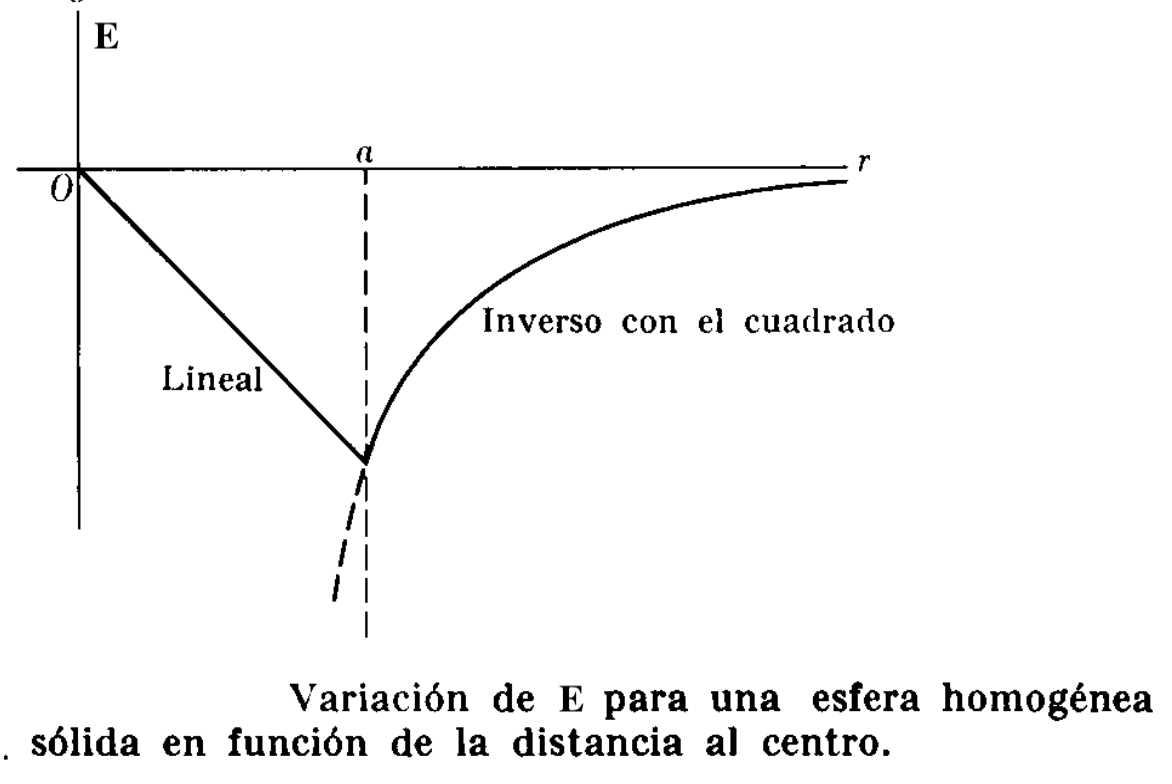
\includegraphics[width=.55\textwidth]{imagenes/imagenes14/T14IM14.png}
\end{figure}
\end{multicols}

Se puede demostrar que el potencial gravitacional en un punto interior de una esfera homogénea de masa $m$ y radio $a$ viene dado por

$V=\dfrac{GM}{2a^3}\left( r^2-3a^2 \right);\quad r<a$ 

y el potencial en el exterior de la esfera, $V=\dfrac{-Gm}{r};\quad r>a$


Por todo lo visto, para el caso de estudio de los efectos de la gravedad entre la Tierra y un satélite ya sabemos la distancia a considerar, la distancia entre sus centros (podemos considerar ambos como puntuales).

\begin{figure}[H]
	\centering
	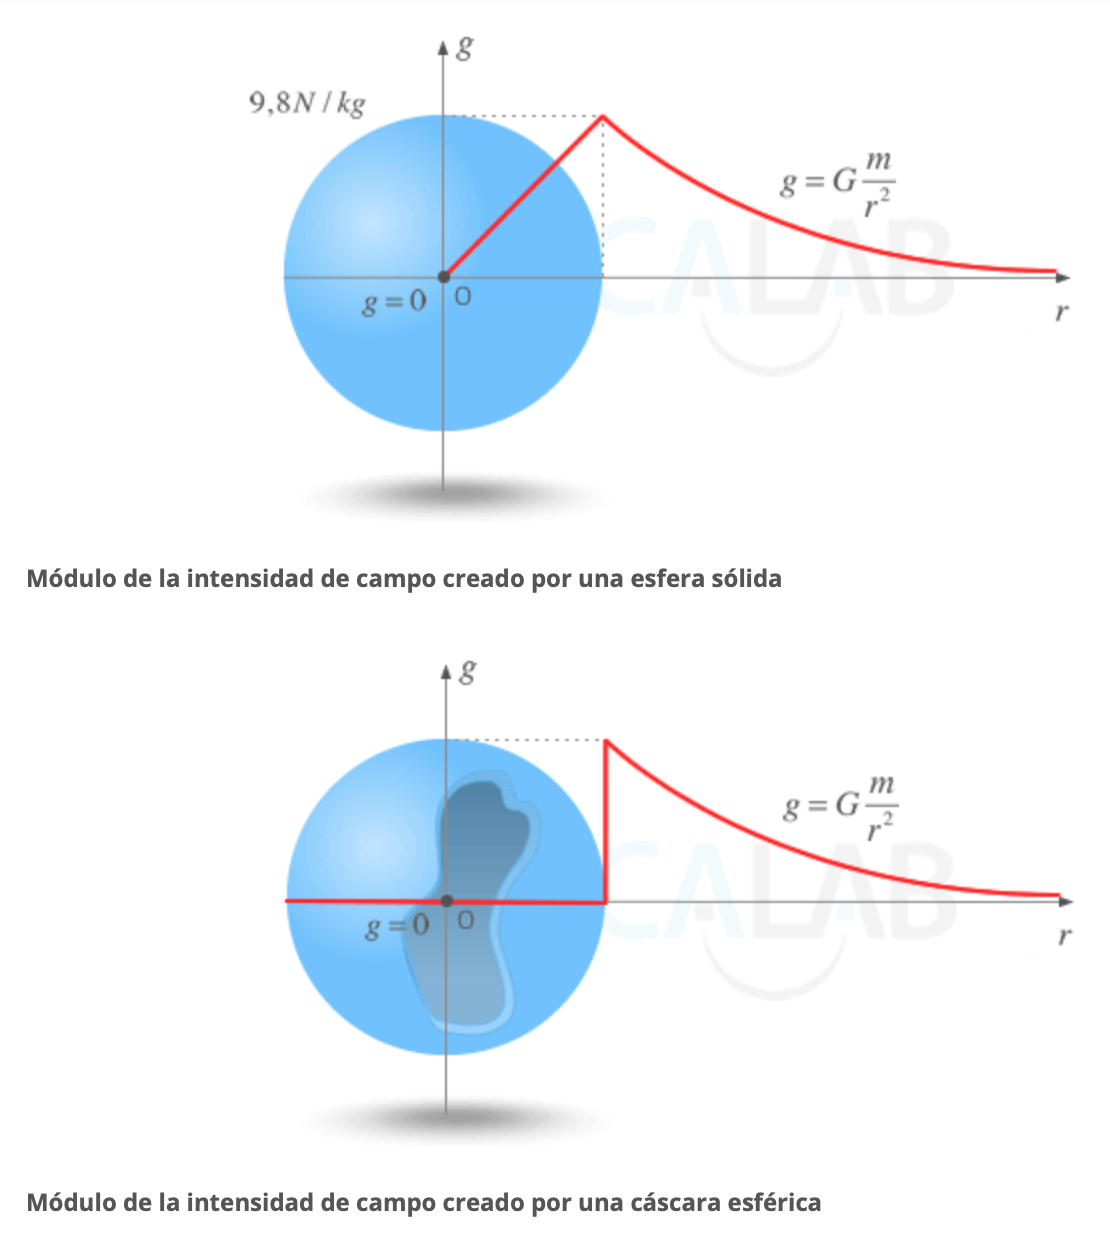
\includegraphics[width=.95\textwidth]{imagenes/imagenes15/T15IM05.png}
	\caption*{--- imagen de `fisicalab.com' ---}
\end{figure}

\section{Experimento de Cavendish. Determinación de $G$}

El experimento de Cavendish o de la \emph{balanza de torsión} permitió obtener implícitamente en 1798 la primera medida de la constante de gravitación universal  $G$  y, con este dato, a partir de la ley de gravitación universal de Isaac Newton y de las características orbitales de los cuerpos del sistema solar, la primera determinación de la masa de los planetas y del Sol. Debe señalarse que Henry Cavendish no calculó esta constante directamente (ya que no la necesitaba para sus mediciones; esto se hizo mucho después, aprovechando sus experiencias), pues su objetivo era determinar la densidad de la Tierra, o, más concretamente, ``pesar la Tierra'', lo que consiguió lograr con una precisión excepcional para su época. Sin embargo, dado que el producto de la constante universal por la masa de la Tierra era conocido desde tiempos de Newton, Henry Cavendish pudo dar la primera estimación del valor de $G$.

\begin{figure}[H]
	\centering
	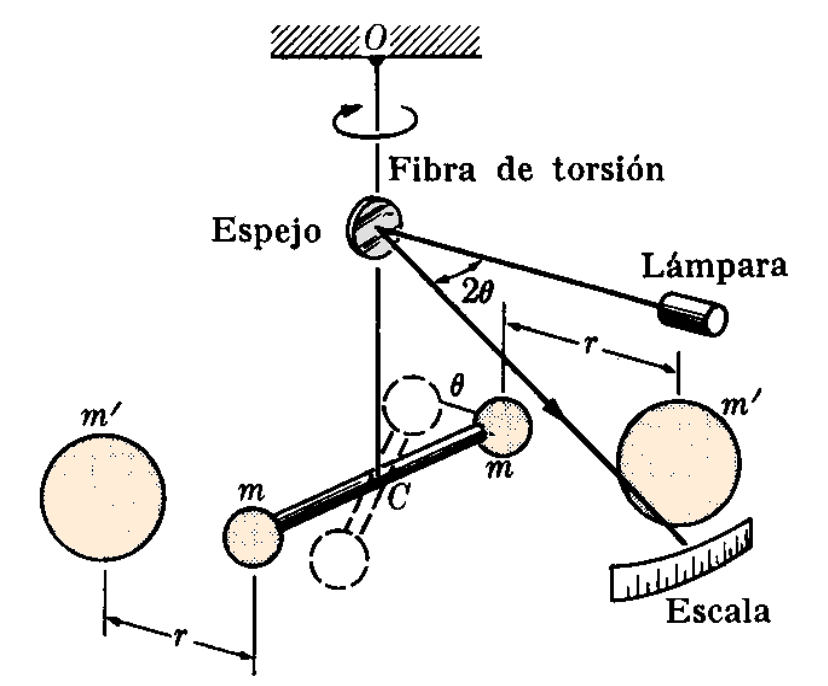
\includegraphics[width=.75\textwidth]{imagenes/imagenes14/T14IM12.png}
\end{figure}

Cuando las masas $m'$ se colocan cerca de las masas $m$, su atracción gravitatoria produce un momento de la fuerza en la barra horizontal que da lugar a una torsión de la cuerda $OC$. El equilibrio se establece cuando los momentos gravitaorio y de torsión se igualan, el de torsión es proporcional a $\theta$ medido por la deflexión de un rayo reflejado en un espejo solidario con la fibra. Repitiendo el experimento a varias distancias $r$ y usando diferentes masas $m$ y $m'$ se puede determinar la constante $G=6.67 \times 10^{-1}\ \mathrm{Nw} \ \mathrm{m}^2 \ \mathrm{kg}^{-2}$.


\section{Masa de la Tierra y de los cuerpos celestes}

\textbf{Masa de la Tierra}: Un cuerpo cualquiera de masa $m$, en las cercanías de la superficie de la Tierra, es atraído por esta por la atracción gravitatoria, su peso:

$F=G\dfrac {Mm}{r^2}=mg \ \to M=\dfrac{g R^2}{G} = 5,97\times 10^{24}\ \mathrm{kg}$.

El radio de la tierra, $R=6371\ \mathrm{km}$, ya lo determinó Eratóstenes en el 276 a.C.


\textbf{Masa de los cuerpos celestes:} Se obtiene aplicando la tercera ley de Keppler, por ejemplo, para la Luna tenemos

$T_L=\dfrac {4 \pi a_L^2}{G(m_L+m_T)}\  \to \ m_L$

La masa de la Tierra se puede comparar con las de otros cuerpos celestes y equivale a $81.3$ veces la masa lunar ($M_L$), $0.00315$ veces la masa de Júpiter, ...
La masa de Júpiter es $M_{Jupiter}=317.83$ veces la masa de la Tierra, $M_\oplus$;  $M_{Saturno}=95.16 M_\oplus$; La masa solar es $M_\odot=332946\ M_\oplus$







\newpage %*****************************************************
\begin{myblock}{ley de gravitación universal}
Es una ley física clásica que describe la interacción gravitatoria entre distintos cuerpos con masa. Fue formulada por Isaac Newton en su libro Philosophiae Naturalis Principia Mathematica, publicado el 5 de julio de 1687, donde establece por primera vez una relación proporcional (deducida empíricamente de la observación) de la fuerza con que se atraen dos objetos con masa. Así, Newton dedujo que la fuerza con que se atraen dos cuerpos tenía que ser proporcional al producto de sus masas dividido por la distancia entre ellos al cuadrado. Para grandes distancias de separación entre cuerpos se observa que dicha fuerza actúa de manera muy aproximada como si toda la masa de cada uno de los cuerpos estuviese concentrada únicamente en su centro de gravedad, es decir, es como si dichos objetos fuesen únicamente un punto, lo cual permite reducir enormemente la complejidad de las interacciones entre cuerpos complejos.

\begin{figure}[H]
	\centering
	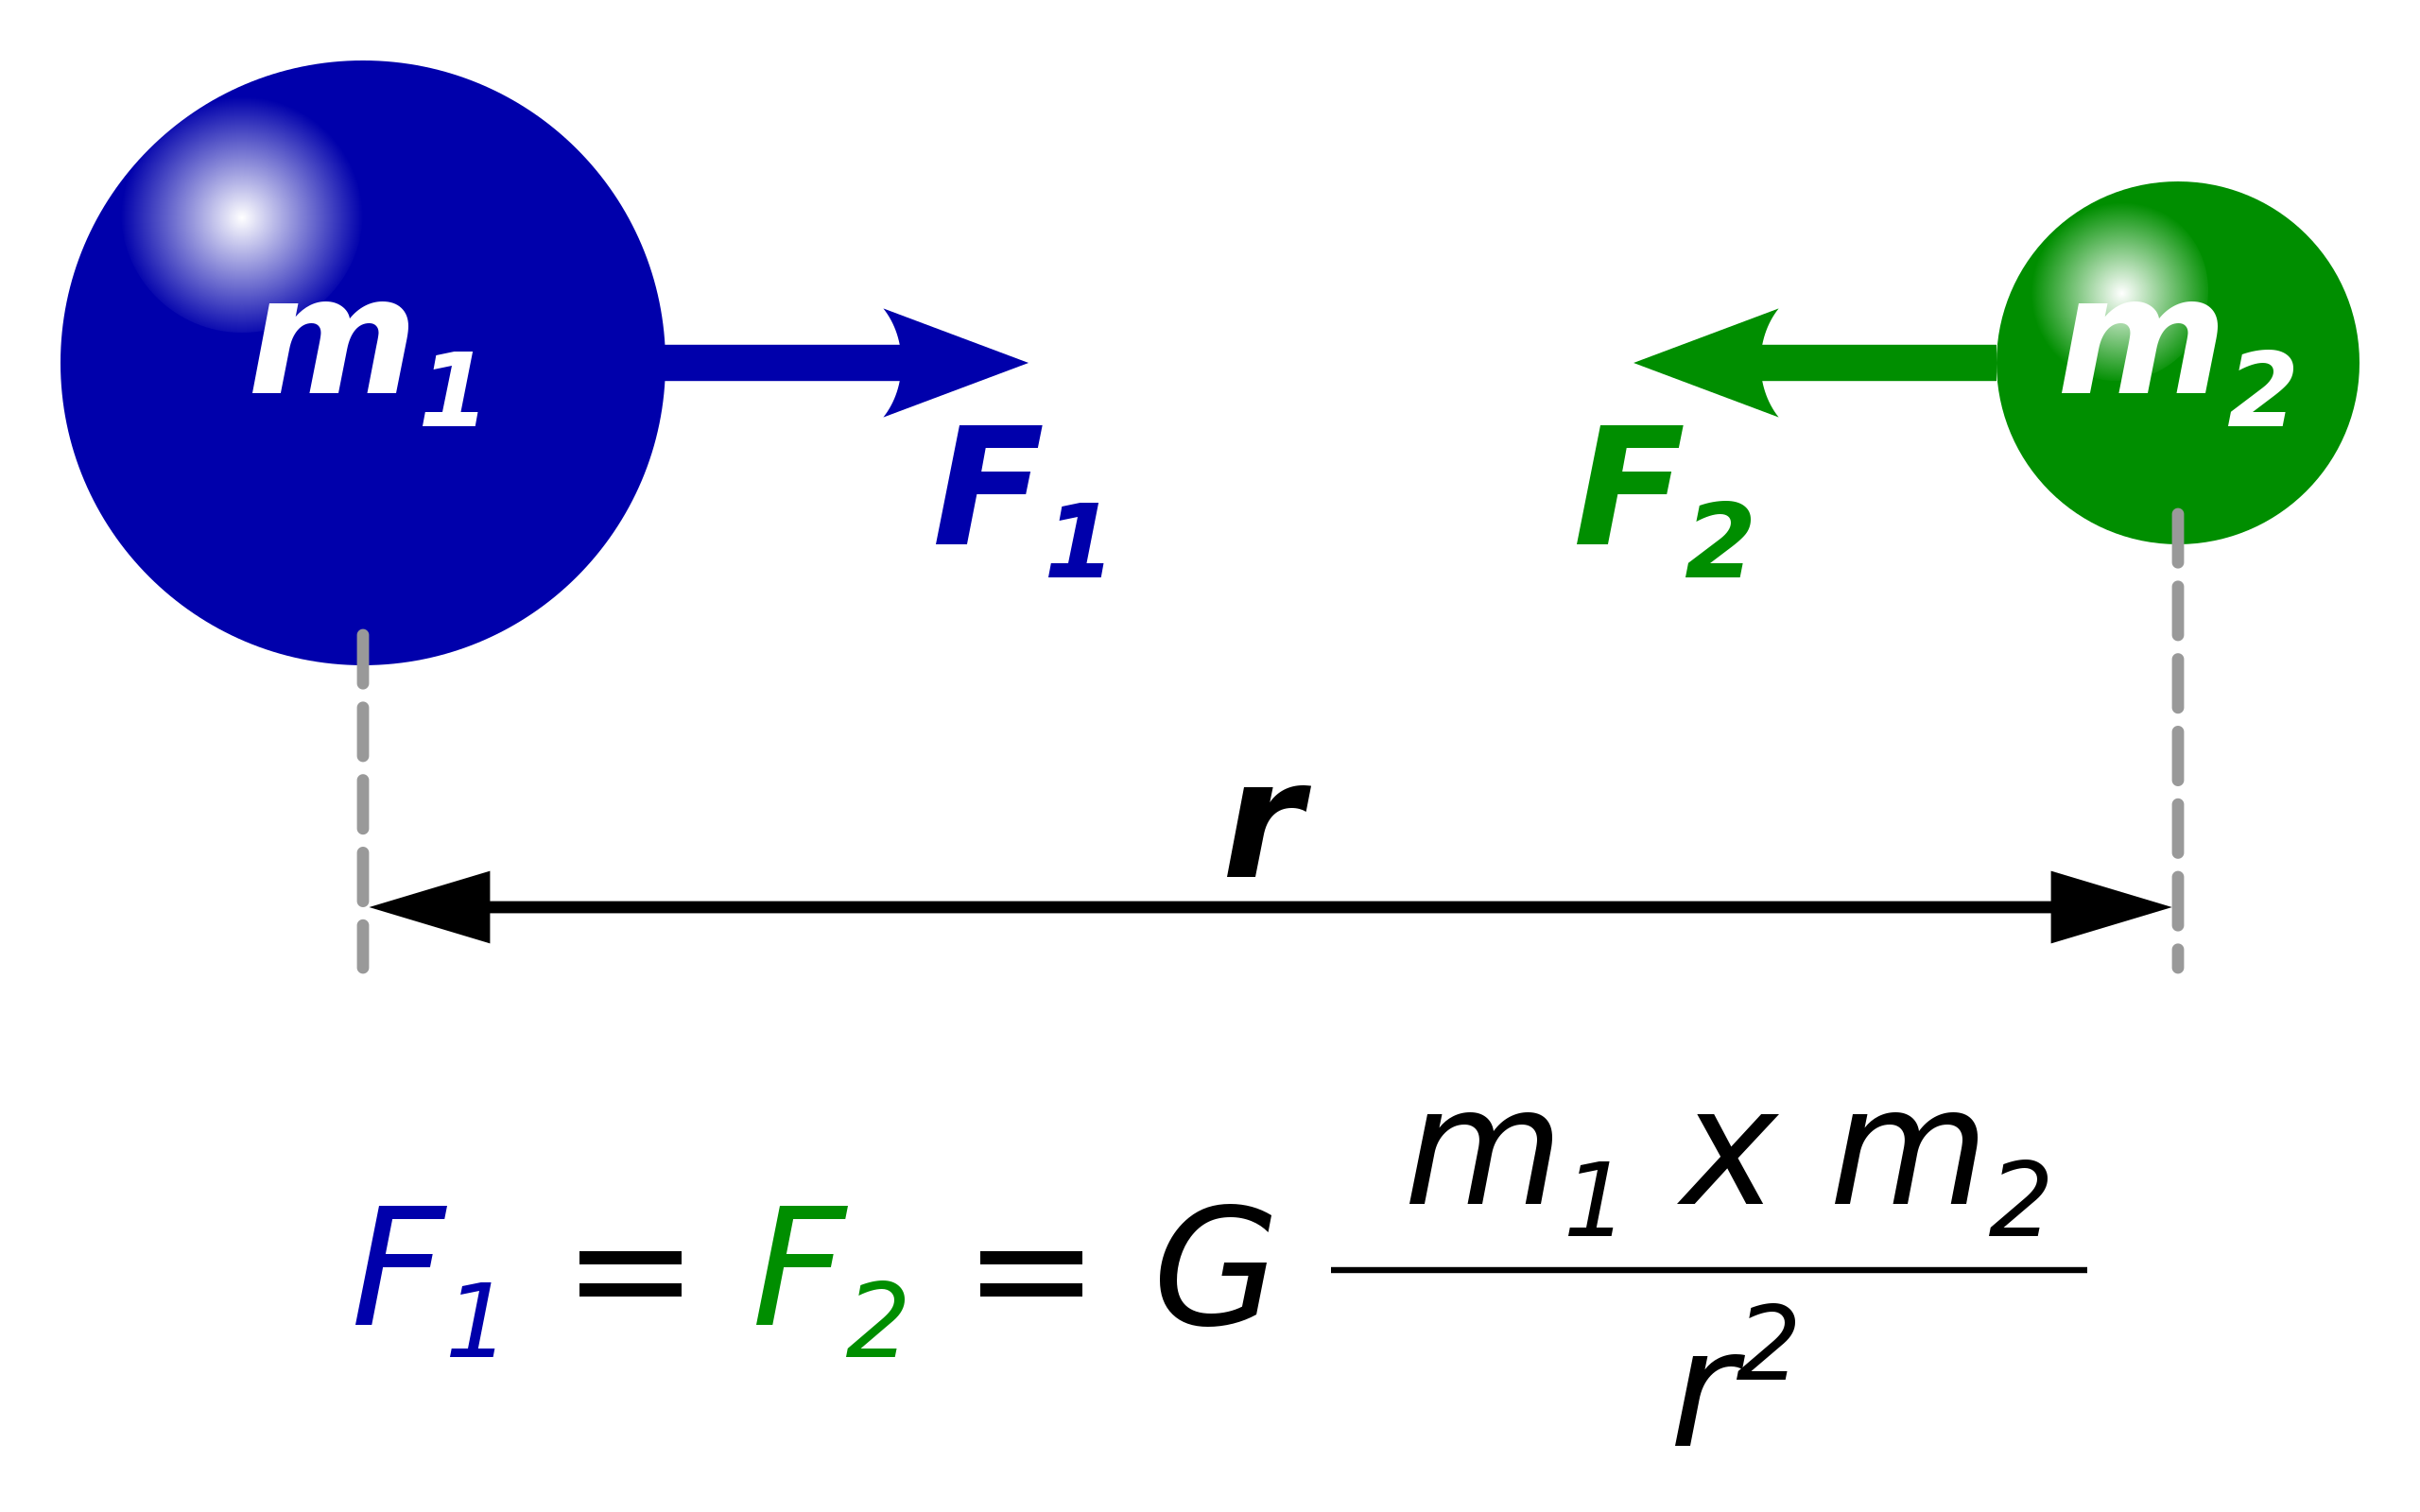
\includegraphics[width=.75\textwidth]{imagenes/imagenes14/T14IM03.png}
\end{figure}

Así, con todo esto resulta que la ley de la gravitación universal predice que la fuerza ejercida entre dos cuerpos de masas $m_1$  y  $m_2$  separados una distancia $r$  es igual al producto de sus masas e inversamente proporcional al cuadrado de la distancia, es decir:
$F=G\dfrac {m_1m_2}{r}$	
\end{myblock}
